\documentclass[11pt,a4paper]{article}
\usepackage[latin1]{inputenc}
\usepackage[english]{babel}
\usepackage{amsmath}
\usepackage{amsfonts}
\usepackage{amssymb}
\usepackage{graphicx}
\usepackage[margin=1in]{geometry}
\usepackage[linesnumbered,noend]{algorithm2e}
\usepackage{tabularx}
\usepackage{hyperref}
\usepackage{xcolor}
\hypersetup{ % Copied from: http://tex.stackexchange.com/a/847/41003
    colorlinks,
    linkcolor={red!50!black},
    citecolor={blue!50!black},
    urlcolor={blue!80!black}
}

% New paragraph = blank line, not indent.
\setlength{\parskip}{0.3cm}
\setlength{\parindent}{0pt}

% Code listings
\usepackage{listings}

\title{An evaluation function for a minimax Draughts player}
\author{
Dennis van der Schagt (0814249)\\
Rob Wu (0787817)
}
\date{\today}


\begin{document}
\maketitle
\newpage
\section*{Abstract}
This report describes a minimax algorithm for an AI agent that plays International Draughts. This algorithm uses a alpha-beta search algorithm to find a good strategy for playing the game. Alpha-beta search is quite a standard algorithm in the field of Artificial Intelligence; the novelty that is presented in this report is the heuristic evaluation function.

\section{The algorithm}
\subsection{Alpha-Beta search}
An implementation of the alpha-beta search algorithm is shown below. Line 3 refers to "the heuristic value", this is elaborated in section \ref{section:heuri}.

\begin{function}[H]
	\DontPrintSemicolon
	\caption{alphabeta(node, remainingDepth, $\alpha$, $\beta$)}
	\KwIn{node, remainingDepth, $\alpha$, $\beta$}
	\If{a player won in node or $remainingDepth = 0$}{
    	\Return{the heuristic value of node}
    }
    \eIf{it's white's turn in node}{
    	\For{each child of node}{
    		$\alpha$:=  maximum of $\alpha$ and alphabeta(child, remainingDepth - 1, $\alpha$, $\beta$)\\
            \If{$beta \leq alpha$}{
				\Return{$\beta$} \tcc*{Beta cut-off}
            }
		}
        \Return{$\alpha$}
    }{ % else
    	\For{each child of node}{
    		$\beta$:= minimum of $\beta$ and alphabeta(child, remainingDepth - 1, $\alpha$, $\beta$)\\
			\If{$\alpha \leq \beta$}{
				\Return{$\alpha$} \tcc*{Alpha cut-off}
			}
		}
		\Return{$\beta$}
	}
\end{function}

\subsection{Heuristic evaluation function}\label{section:heuri}
We intentionally kept our evaluation function simple and fast. Keeping it simple makes it easier to understand what is going on and thus easier to improve the magic numbers. Because of the simple evaluation function we also had an easier time fixing a bug we had in our alpha-beta algorithm. Keeping the function fast allows us to look forward as many turns as possible in the given time.

The evaluation function returns a single integer value which reflects the state of the game. A negative value means that black is likely going to win, whereas a positive value means that white will probably win. When the game state is such that one of the players is certainly going to win, the returned value is an extreme value. E.g. if black will certainly win from white, then the returned value is the maximum representable negative integer.

If it is not set in stone which player will win, then the score is calculated from the number of pieces on the board and their position.
We assume that the number of pieces is the most important indicator of success, so this feature is the primary score component. To make sure that this primary choice is always respected irrespective of the position scores, the scores are chosen such that the sum of the position scores can never exceed the smallest unit of the piece count score.

The piece score modifier is used to value the pieces that are on the board. For this part we only look at the kind of piece, white or black, uncrowned or king. We give a value of $1000$ to a white uncrowned piece. On advice of dr.ir. J.W. Wesselink we decided to value kings thrice as high as an uncrowned piece, so a white king is worth $3000$. This makes sure our player will work toward getting a king without giving up too many uncrowned pieces for that goal. The values of the black pieces are the opposite of the values of the white pieces, as we want to have a symmetric evaluation function.

The position score modifier associates a value to a piece depending on their row position. The closer a piece is to the other side of the board, the higher its bonus score. This criteria exists to encourage reaching the other end in order to get a king, even when the AI agent cannot look that deep in the game tree. Because this criteria only exists to stimulate becoming a king, the bonus is only added to uncrowned pieces. Note that the piece count takes precedence over position, so the agent will not unconditionally move pieces forwards in an attempt to get a piece to the other end, because this action would negatively affect the piece count (i.e. blindly moving forward allows the opponent to kill a piece).

To avoid moving too many pieces to the other side of the board, the first row will get a higher bonus score than the first few rows, to encourage pieces to stay home. This allows them to prevent opposing pieces from being a king.

A way to implement this bonus system is by awarding one bonus point to a piece for moving one row forwards. A disadvantage of this mechanism is that it does not differentiate between a piece that is already close to the end, and a piece that is still at first rows. To distinguish between both situations, the list of bonus scores for each row is a Fibonacci sequence. The final list of bonus scores is shown in table \ref{table:bonusscore}. There are at most 20 pieces per player. The maximum score for a piece is $31$, so the maximum bonus is not higher than $20\times 31 = 620$, which is well below $1000$ (the piece count score for an uncrowned piece).

\begin{table}[ht]
\begin{tabularx}{\linewidth}{l|l|X}
row & score & comment \\
\hline
1 & 10 & Staying home is preferable to moving one forward, in order to defend against incoming pieces from the opponent. \\
2 & 1 & \\
3 & 2 & = more than 1 \\
4 & 3 & = 1 + 2\\
5 & 5 & = 2 + 3\\
6 & 8 & $\dots$\\
7 & 13 & \\
8 & 21 & \\
9 & 31 & \\
10 & 0 & A piece at the end is already a king. There's no need to associate a score with a piece at the last row, because this case does not occur. \\
\end{tabularx}
\caption{Bonus scores for piece position.}\label{table:bonusscore}
\end{table}

\section{Results}
Our player did fairly well in the tournament, especially given the fact that our evaluation function contained an error. As a result of this error the white player focussed more on keeping his pieces on the back line than on getting a material advantage. Because of that we lost one match of the group phase and consequently we did not qualify for the quarter finals. After finding and fixing the error we reran all the matches, playing on the white side, as well as the black side. This time we won all those matches. Then we continued testing by playing against the winner of the tournament (player 42/Poro\_Plank). We lose consistently when playing on the black side but when playing as white most of our games result in a win [\ref{fig:win42}] or a draw [\ref{fig:draw42}].

Our player plays relatively good for the limited rules we use in the evaluation function. The number of moves that we can look ahead probably plays a more significant role. Throughout the game our player can look between 7 and 9 moves ahead (using 2 seconds each move). We did not optimize much in the alpha-beta search. If we would ever want to improve our player we could start by ordering the moves. In that way we could probably prune more of the tree and consequently look further ahead in the more interesting parts of the search tree. More improvements could be made in the evaluation function. One such improvement, which we didn't have enough the time for, is looking to the number of neighbours of every piece.

\section{Reproducing the results}
Following are the steps required to reproduce our results:
\begin{itemize}
\item Download the tournament NetBeans project from \url{http://www.win.tue.nl/~wstahw/edu/2ID90/tournament-2015.zip} and unzip it
\item Download our player plugin's NetBeans project from Peach and build it
\item Copy the jar file from our player project to the plugins folder of the tournament project, thereby replacing our old player
\item Run the tournament project
\item Select our player (AlphaBetaPlayer) and one of the other players
\item Run the competition
\end{itemize}
Keep in mind that results can vary with the time given per move. We ran all test games with 2 seconds per move.

\section{References}
\url{http://www.cs.columbia.edu/~devans/TIC/AB.html}
%\url{http://stackoverflow.com/a/15626976/1928529} of \url{http://en.wikipedia.org/wiki/Alpha%E2%80%93beta_pruning#Pseudocode} (Voor alphabeta pseudocode)

\section{Contributions}

\section{Appendix}
\begin{figure}[h!]
\centering
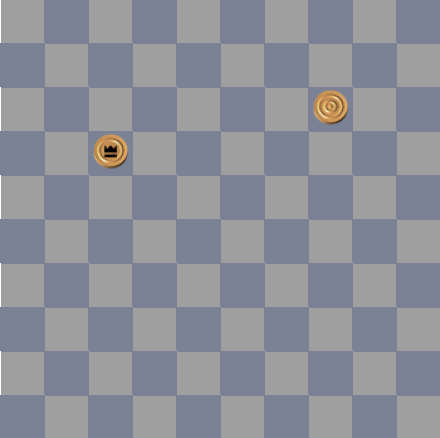
\includegraphics{win_with_42.png}
\caption{Final result of a game in which we played as white against the winner of the tournament.}
\label{fig:win42}
\end{figure}
\begin{figure}[h!]
\centering
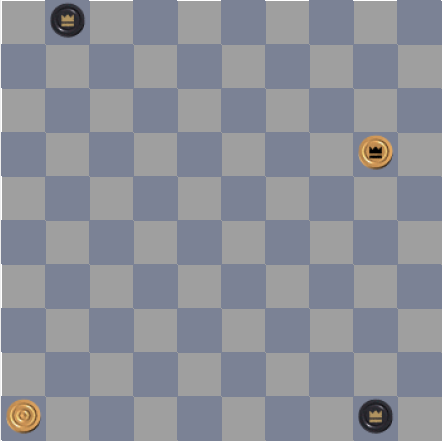
\includegraphics{draw_with_42.png}
\caption{One of the many draws with the winner of the tournament.}
\label{fig:draw42}
\end{figure}

\end{document}














